\documentclass{article}
\usepackage{fullpage}
\usepackage{biblatex}
\usepackage{graphicx}
\usepackage{listings}
\bibliography{refs.bib}
\setlength{\parskip}{4pt}
\setlength{\parindent}{0pt}
\title{Advanced databases: Homework 2}
\author{Leendert Dommicent and Jorn Van Loock}
\begin{document}
\maketitle
\section{Merging the ontologies}
The merging of the ontologies was done manually. Our own ontology was quite small so doing it manually seemed the best and fasted solution. In figure 1 you can find the EER diagram of our ontology from the previous assignment. Now follow the steps which we followed to merge the ontology in chronological order.
\begin{itemize}
\item We started by taking the given factbook ontology.
\item Next we added our versions of \textit{Country} and \textit{Government type} and added all the declarations of the corresponding classes in the factbook ontology to this two classes. We also changed the declaration of our \textit{Name} property from equivalent class to superclass, because this is a shared variable who is used by many classes. This was an error in our previous ontology. We ofcourse deleted the original \textit{Country} and \textit{Government type} classes afterwards.
\item We removed \textit{Code} from the object properties because it was already in the data properties.
\item \textit{GeographicCoordinates} were moved to the data properties because we see this as a property instead of a relation to a coordinate individual.
\item We decided to take their religion ontology because it could handle percentages and ours couldn't.
\item We renamed their object relation \textit{Government} to our relation \textit{hasGovernment}.
\item We removed the class \textit{latlon} because we use the \textit{GeographicCoordinate} data property of the factbook ontology.
\item We added all our other remaining object relation of our ontology.
\item We added our data relations \textit{date}, \textit{id} and \textit{numberOfFatalities}.
\item We used the \textit{name} data property of the factbook ontology for our ontology.
\item We changed the types of all the data properties to strings. The reason for this is given below.
\end{itemize}
The resulting ontology is the ontology we populated.
\begin{figure}
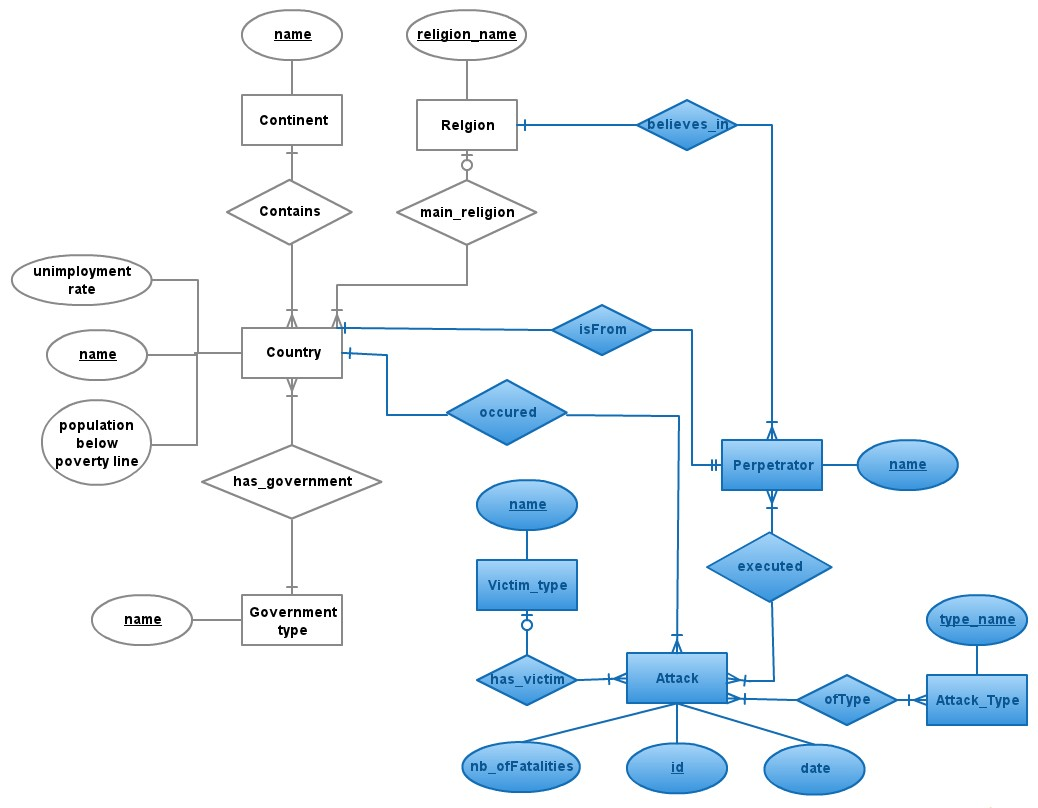
\includegraphics[width=1\textwidth]{TerroristAttacks.jpg}
\caption{Our own ontology from the first assignment}
\label{fig:ontology}
\end{figure}
\section{Automate the population}
To populate the ontologies we had to use some kind of automation because the dataset was too large to do it manually. In subsection 2.1 we describe how we parsed the html pages of the CIA Factbook. In subsection 2.2 we describe how we parsed the csv file of the Terrorist Attack database. Finally in subsection 2.3 we explain how we managed to get all this data in the existing OWL ontology.
\subsection{Parsing the CIA Factbook}
\label{sec:factbook}
Because the factbook is a website and the content is only available in html we had to parse the html.
To parse all the html pages we used the java library \textit{Jsoup}\cite{jsoup}. We can give a url to the library and the html-code will be fetched.
\par
We started by giving "https://www.cia.gov/library/publications/the-world-factbook/print/textversion.html" to the library to parse all the countries and URL's to the countries.
For each country the page is parsed in an automatic way. We searched for a pattern to find the names and the values of the properties.
If you take a look at a page of a country you'll see the blue titles (like \textit{Location}), we call this the maintitles; and their content (like \textit{Southern Asia, north and west of Pakistan, east of Iran}).
Sometimes inside the content there is a new property. Take a look to maintitle \textit{Area}, inside the content there are new subtitles \textit{total}, \textit{land} and \textit{water}. We took the subtitle and put it in front of the maintitle.
We created a class \textit{FilteredProperty} containing a title and a value and we set each title to camelcase:
\\\textit{String title = "location"; String value = "Southern Asia, north and west of Pakistan, east of Iran"}
\\\textit{String title = "waterArea"; String value = "0 sq km"}
\\We can now have all the html-properties parsed and make them available as instances of \textit{FilteredProperty}. We now need to map them to the ontology relations and properties.
\par
For the mapping we created an \textit{enum} containing all the relations(\textit{RelationType}) and an \textit{enum} containing all the properties(\textit{PropertyType}) of the ontology with the exact same name. We created the classes \textit{Property} and \textit{Relation}.
They take the necessary arguments: A \textit{property} belongs to an individual, holds a \textit{PropertyType} and has a value.
A \textit{relation} holds a \textit{RelationType} and is between two individuals which are from a specific class.
\par
First, we compared the parsed title of every \textit{FilteredProperty} to the enumeration of the properties. If they are the same (like \textit{waterArea}) an instance of \textit{Property} can be created.
Due to setting the title as camelcase much things directly correspond to the propertyname of the OWL-ontology.
Ofcourse this was not the case for all properties, thus we created a convertor that renames the parsednames that weren't found in \textit{PropertyType} to the right \textit{PropertyType}. This had to be done for all the remaining properties such that from now on for every property an instance of \textit{Property} can be made:
\begin{lstlisting}
...
if(htmlProperty.getProperty().equals("maritimeClaims"))
	htmlProperty.renameProperty("maritimeClaim");
...
\end{lstlisting}
Second, the relations had to be done. Also in the convertor we created the instances of \textit{Relation} for the remaining instances of \textit{FilteredProperty} that are relations and not properties (the properties are already taken out in the previous step).
The mapping to the right \textit{RelationType} had to be done for each parsed title that is a relation.
\begin{lstlisting}
...
if(htmlProperty.getProperty().equals("naturalResources")){
	String[] resources = htmlProperty.getValue().split(", ");
	for(String resource : resources){
		resource = convertToValid(resource);
		Relation r = new Relation(country.getIndividualName(), 
			RelationType.naturalResource, resource, "NaturalResource", 
			"Country");
		country.addRelation(r);
		Property p = new Property(resource, PropertyType.name, resource);
		country.addProperty(p);
	}
	return true;
}
...
\end{lstlisting}
At the and we have a set \textit{Relation} instances and \textit{Property} instances with enough information in it to be added the to the ontology.
\par
You can find the resulting code in the packages \textit{parser.factbook} and \textit{concept} in the GitHub project\cite{githubproject}.

\subsection{Parsing the Terrorist Attack database}
\label{sec:terrorist_db}
The content of the terrorist database came in .csv format. Because .csv is a popular data format we were very confident to find a good Java parser to parse this file. We found the parser Super CSV\cite{supercsv}. Super CSV can parse .csv files and gives back a \textit{HashMap} for every record that maps the field names onto the values. Everything is parsed as a \textit{String} and handled accordingly.\par
You can find the resulting code in the class \textit{TerroristParser} in the GitHub project\cite{githubproject}.
\subsection{Writing to OWL}
\label{sec:writ_owl}
Now that we have parsed all the data we have to write it to the OWL ontology. Doing this manually by writing directly to the OWL file would be a lot of work and would be very error prone. We decided to search for a Java library that would do this for us.\par
The first Java library we tried was the one of Prot\'eg\'e. However the development of this API had stopped at the beginning of version 4 so we decided not to use this API.\par
Next we found the OWL API\cite{owlapi}. This api has a lot of features to read and write data to OWL ontologies. The only drawback was that the version for OWL 1 didn't had all the functionality we needed so we decided to use the version for OWL 2. This version didn't had any problems with reading the given OWL 1 ontology.\par
We then wrote some methods to add individuals, object relations and data relations. One drawback is that all the data properties are strings, because we parse everything as strings. This was the easiest solution and was good enough by our opinion for this exercise. We changed the ontology slightly by making all the data properties strings. You can find the resulting code in the class \textit{OwlHandler} in our GitHub project\cite{githubproject}.
\section{Conclusion}
In this report we described how we merged our ontology manually with the given factbook ontology. Next we explained how we wrote the program to populate this ontology automatically.
\printbibliography
\end{document}
